\begin{figure}
    \centering
    %\vspace{-1em}
    \begin{subfigure}[b]{0.4\linewidth} % 40% width
        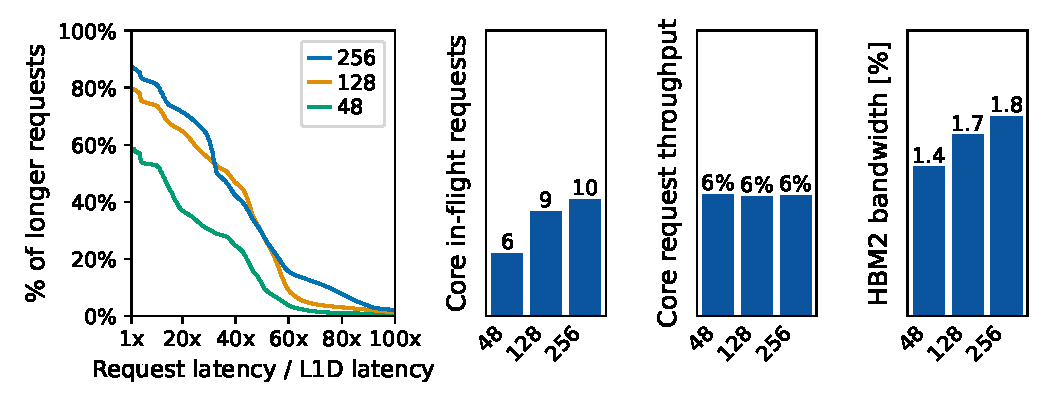
\includegraphics[width=\linewidth,trim=0 0 290 0,clip]{img_embedding_implications_arxiv.pdf}
        \vspace{-2em}
        \caption{\texttt{arxiv}}
        %\vspace{0.5em}
        %\label{fig:ltu-arxiv}
    \end{subfigure}
    \begin{subfigure}[b]{0.4\linewidth} % 40% width
        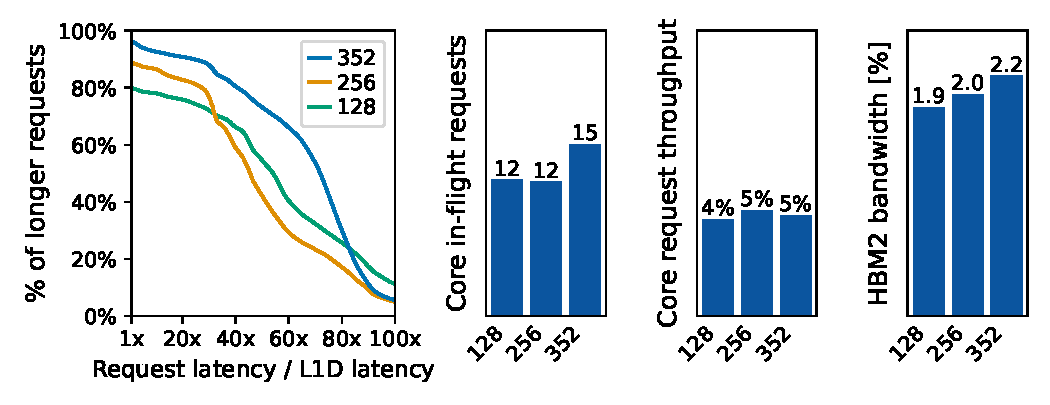
\includegraphics[width=\linewidth,trim=0 0 290 0,clip]{img_embedding_implications_mag.pdf}
        \vspace{-2em}
        \caption{\texttt{mag}}
        %\vspace{0.5em}
        %\label{fig:ltu-mag}
    \end{subfigure}
    \begin{subfigure}[b]{0.4\linewidth} % 40% width
        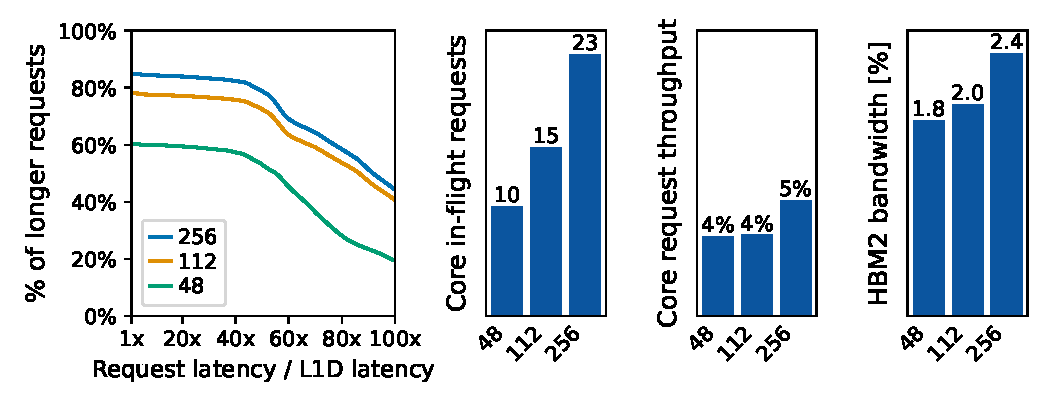
\includegraphics[width=\linewidth,trim=0 0 290 0,clip]{img_embedding_implications_products.pdf}
        \vspace{-2em}
        \caption{\texttt{products}}
        %\vspace{0.5em}
        %\label{fig:ltu-products}
    \end{subfigure}
    \begin{subfigure}[b]{0.4\linewidth} % 40% width
        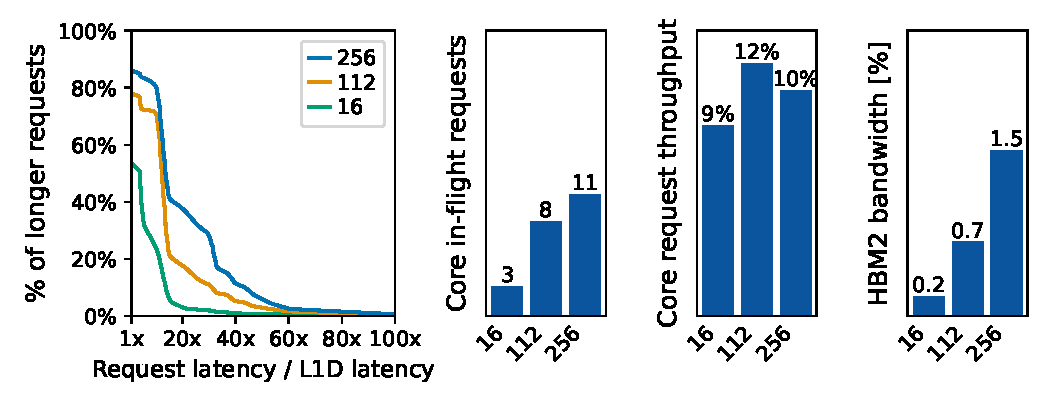
\includegraphics[width=\linewidth,trim=0 0 290 0,clip]{img_embedding_implications_proteins.pdf}
        \vspace{-2em}
        \caption{\texttt{proteins}}
        %\vspace{0.5em}
        %\label{fig:ltu-proteins}
    \end{subfigure}
    %\vspace{-2em}
    \caption[Load-to-use latency of embedding lookups on CPU.]{Load-to-use latency of GNN embedding lookups. The y-axis shows the percentage of requests longer than the corresponding value on the x-axis, which is computed as request latency relative to the latency of accessing the L1D cache. Overall, a large fraction of embedding lookups in GNN models take orders of magnitude longer than L1D accesses. For \texttt{products}---the dataset with the lowest locality---more than 74\% of memory requests (y-axis) are 10$\times$ longer than an L1D access (x-axis), and 40\% are more than 100$\times$ longer, as they need to reach HBM.}
    \label{fig:ltu-gnn}
\end{figure}

\begin{figure}
    \centering
    %\vspace{-1em}
    \begin{subfigure}[b]{0.45\linewidth} % 40% width
        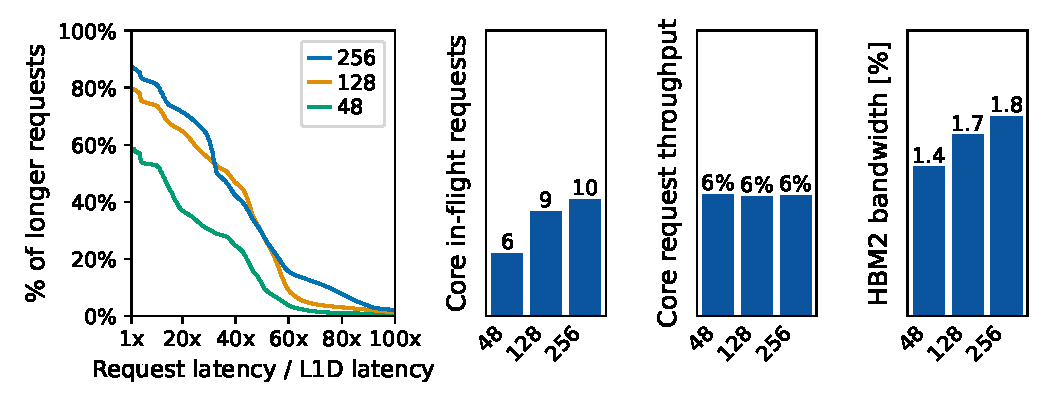
\includegraphics[width=\linewidth,trim=210 0 0 0,clip]{img_embedding_implications_arxiv.pdf}
        \vspace{-2em}
        \caption{\texttt{arxiv}}
        %\vspace{0.5em}
        %\label{fig:ltu-arxiv}
    \end{subfigure}
    \hspace{1cm} % <-- increase this to spread them
    \begin{subfigure}[b]{0.45\linewidth} % 40% width
        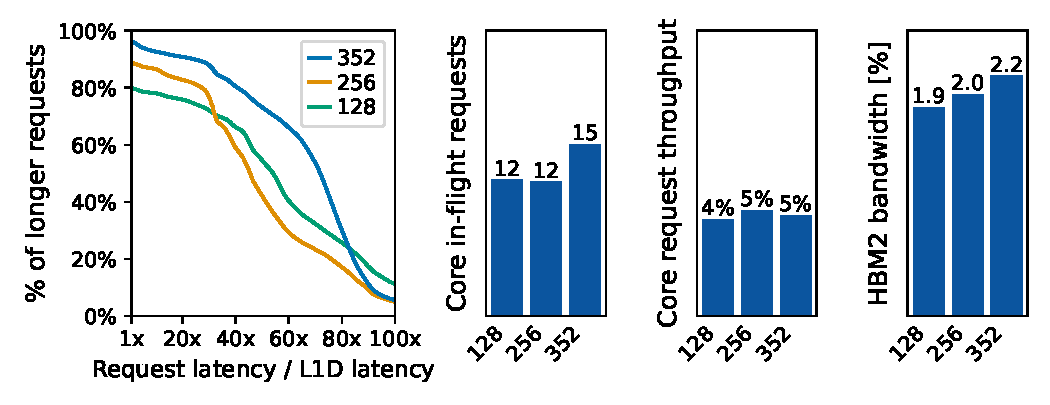
\includegraphics[width=\linewidth,trim=210 0 0 0,clip]{img_embedding_implications_mag.pdf}
        \vspace{-2em}
        \caption{\texttt{mag}}
        %\vspace{0.5em}
        %\label{fig:ltu-mag}
    \end{subfigure}
    \begin{subfigure}[b]{0.45\linewidth} % 40% width
        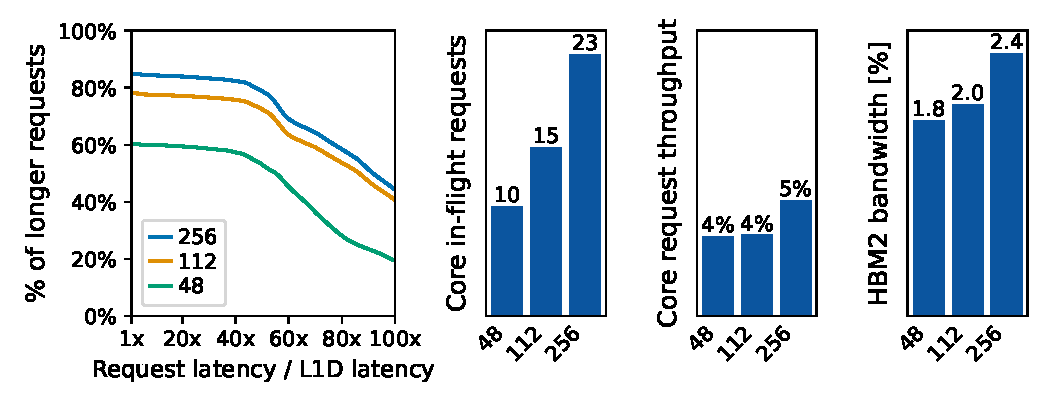
\includegraphics[width=\linewidth,trim=210 0 0 0,clip]{img_embedding_implications_products.pdf}
        \vspace{-2em}
        \caption{\texttt{products}}
        %\vspace{0.5em}
        %\label{fig:ltu-products}
    \end{subfigure}
    \hspace{1cm} % <-- increase this to spread them
    \begin{subfigure}[b]{0.45\linewidth} % 40% width
        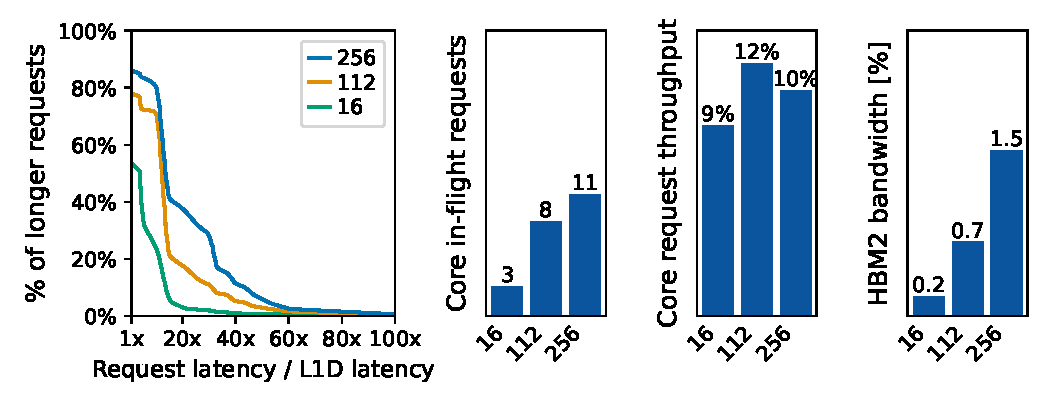
\includegraphics[width=\linewidth,trim=210 0 0 0,clip]{img_embedding_implications_proteins.pdf}
        \vspace{-2em}
        \caption{\texttt{proteins}}
        %\vspace{0.5em}
        %\label{fig:ltu-proteins}
    \end{subfigure}
    %\vspace{-2em}
    \caption[Architectural implications of embedding lookups on CPU.]{Architectural implications of long embedding lookups on an off-the-shelf CPU core. Bars correspond to different embedding sizes. The leftmost plot shows the average number of in-flight memory requests tracked by the core. The middle plot shows request throughput utilization, computed as actual request throughput relative to the peak throughput of one request per cycle. The rightmost plot shows memory bandwidth utilization. As shown in the leftmost plots, the higher the average latency, the higher the number of in-flight requests tracked by the core. However, because of their limited memory-level parallelism, CPU cores can only track a few requests before the whole pipeline stalls. As shown in the middle plots, due to these stalls, the core issues memory requests at a fraction of its peak throughput of one request per cycle. Even \texttt{proteins}---the dataset with the highest locality---only achieves up to 12\% throughput. As shown in the rightmost plots, this results in low HBM per-core utilization. Even a low-locality dataset like \texttt{products}---with the majority of accesses reaching HBM---utilizes up to 2.4\% bandwidth. Overall, off-the-shelf traditional cores are not optimized for long memory accesses.}
    \label{fig:embedding-implications}
\end{figure}
